\documentclass[
  11pt,
  letterpaper,
   addpoints,
  % answers
  ]{exam}

\usepackage{../exercise-preamble}
\usepackage{multicol}
\begin{document}

\noindent
\begin{minipage}{0.47\textwidth}

\includegraphics[width=\textwidth]{../fcfm_die}
\end{minipage}
\begin{minipage}{0.53\textwidth}
    
\begin{center} 
\large\textbf{Análisis y Diseño de Circuitos Eléctricos} (EL3101-2) \\
\large\textbf{Clase auxiliar 1} \\
\normalsize Prof.~Santiago Bradford V.\\
\normalsize Prof.~Aux.~Erik Saez A. - Rodrigo Catalán\\
             - Byron Castro R.
\end{center}
\end{minipage}

\vspace{0.5cm}
\noindent
\vspace{.85cm}


\begin{questions}
    %%%%%%%%%%%%%%%%%%%%%%%%%%%%
    \question     
    El voltaje que circula a través de un elemento de circuito es $v(t) = 20(1 - \exp(-8t))$ V cuando $t \geq 0$ y $v(t) = 0$ cuando $t < 0$. La corriente en este elemento es $i(t) = 30\exp(-8t)$ mA cuando $t \geq 0$, e $i(t) = 0$ cuando $t < 0$. La corriente y el voltaje del elemento se apegan a la convención pasiva. Especifique la potencia que este dispositivo puede ser capaz de absorber de manera segura.
    %%%%%%%%%%%%%%%%%%%%%%%%%%%%
    \begin{solution}
        Se busca obtener la potencia a la que el dispositivo es capaz de absorver de manera segura. Se tiene que:
        \begin{equation}
            v(t) =
            \begin{cases} 
            20(1 - e^{-8t}) \text{ V}, & t \geq 0 \\ 
            0, & t < 0 
            \end{cases}
            \end{equation}
            
            \begin{equation}
            i(t) =
            \begin{cases} 
            30e^{-8t} \text{ mA}, & t \geq 0 \\ 
            0, & t < 0 
            \end{cases}
         \end{equation}
        La potencia instantánea se puede obtener como:
        \begin{equation}
            p(t) = v(t) \cdot i(t) =
            \begin{cases} 
            20(1 - e^{-8t}) \cdot 30e^{-8t} \text{ mW}, & t \geq 0 \\ 
            0, & t < 0
            \end{cases}
        \end{equation}
        Luego esta potencia sera maxima en presencia de maximos locales o globales, por tanto se busca dichos puntos.
        \begin{align}
            \frac{dp(t)}{dt} &= 0 \\
            \frac{d}{dt} \left( 20(1 - e^{-8t}) \cdot 30e^{-8t} \right) &= 0\\
            \frac{d}{dt} \left( (1 - e^{-8t}) e^{-8t} \right) &= 0 \\
            \frac{d}{dt} \left( e^{-8t} - e^{-16t} \right) &= 0\\
            -8 e^{-8t} + 16 e^{-16t} &= 0 \\
            - e^{-8t} + 2 e^{-16t} &= 0\\
            \frac{e^{-8t}}{e^{-16t}} &= 2\\
            e^{8t} &= 2\\
            8t &= \ln(2)\\
            t &= \frac{\ln(2)}{8} \approx 0.01
        \end{align}
        De esta manera se obtiene que reemplazando en la ecuacion de potencia:
        \begin{equation}
        p\left(t= \frac{ln(2)}{8}\right) \approx 150 \text{ mW}
        \end{equation}
        \begin{center}
            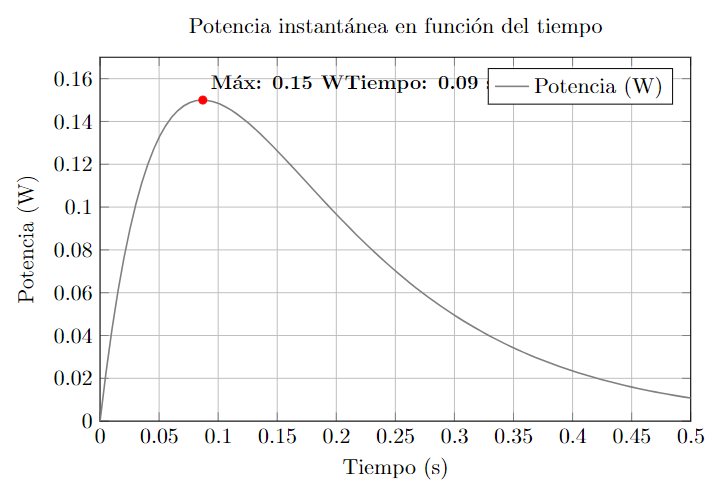
\includegraphics[width=0.8\textwidth]{Auxiliar_1_12}
            \captionof{figure}{Grafico de la potencia instantánea en funcion del}
        \end{center}
    \end{solution}
    %%%%%%%%%%%%%%%%%%%%%%%%%%%
    \question  Para el circuito de la figura:

    \begin{enumerate}
        \item El valor de R2 respecto a R1 que maximiza la potencia disipada en R2.
        \item Qué ocurre con la potencia si el valor de R2 es muy alto (Aprox. a $\infty$).
        \item Qué ocurre con la potencia si el valor de R2 es muy bajo (Aprox. a 0).
    \end{enumerate}
    \begin{center}
        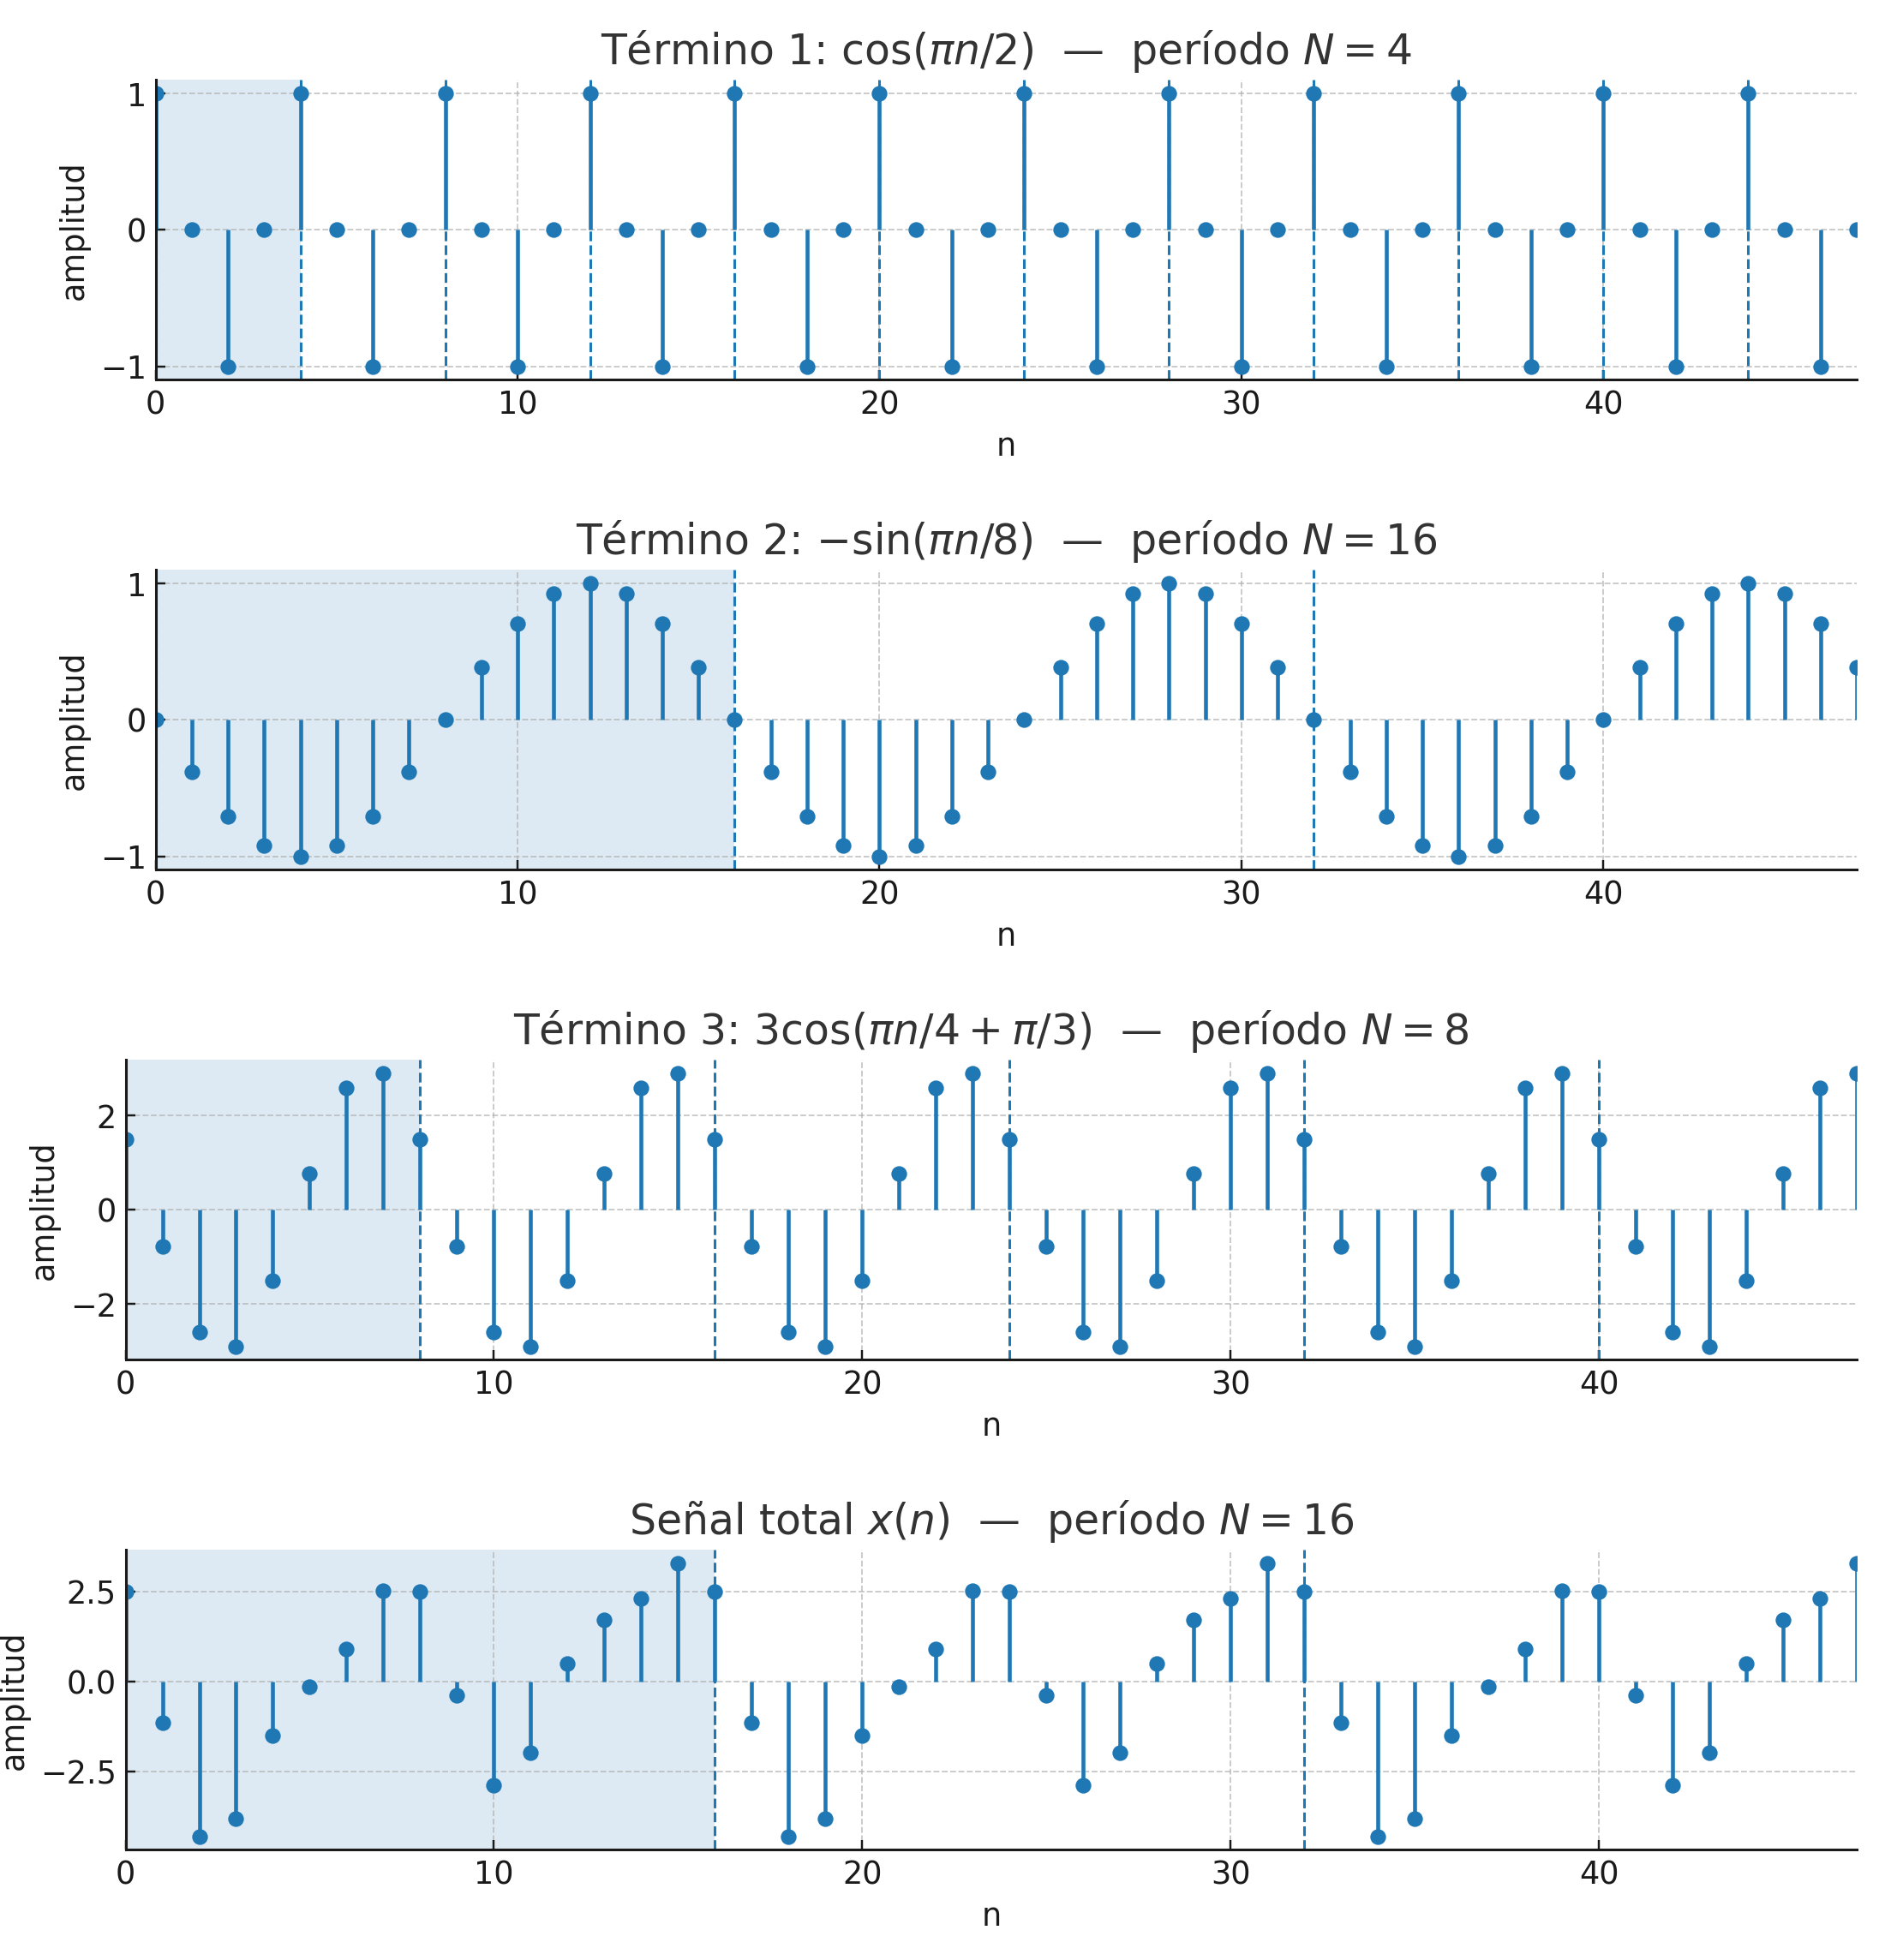
\includegraphics[width=0.4\textwidth]{Auxiliar_1_1}
        \captionof{figure}{Esquema del circuito}
    \end{center}
    %%%%%%%%%%%%%%%%%%%%%%%%%%%
    \begin{solution}
        \begin{enumerate}
            \item Se busca obtener el valor de $R_2$ respecto a $R_{1}$ que maximiza la potencia disipada en $R_2$, por lo tanto:
            \begin{align}
            V - V_{R1} - V_{R2} &= 0\\
            V &= V_{R1} + V_{R2}\\
            V &= R_{1} \cdot I_{1} + R_{2} \cdot I_{1}\\
            I_{1} &= \frac{V}{R_{1} + R_{2}}
            \end{align}
            Luego reemplazando sobre la potencia disipada en $R_{2}$:
            \begin{align}
                P_{R2} &= V_{R2} \cdot I_{1}\\
                &= R_{2} \cdot I_{1}^{2}\\
                &= R_{2} \cdot \left( \frac{V}{R_{1} + R_{2}} \right)^{2}
            \end{align}
            Para cumplir la condicion de maximo se deriva respecto a $R_{2}$ y se iguala a 0, tal que:
            \begin{align}
                \frac{dP_{R2}}{dR_{2}} &= 0\\
                \frac{d}{dR_{2}} \left( R_{2} \cdot \left( \frac{V}{R_{1} + R_{2}} \right)^{2} \right) &= 0\\
                \frac{1}{(R_{1} + R_{2})^{2}} - \frac{2R_{2}}{(R_{1} + R_{2})^{3}} &= 0\\
                \frac{1}{(R_{1} + R_{2})^{2}} &= \frac{2R_{2}}{(R_{1} + R_{2})^{3}}\\
                1 &= \frac{2R_{2}}{(R_{1}+R_{2})}\\
                R_{1} + R_{2} &= 2R_{2}\\
                R_{1} &= R_{2}
            \end{align}
            De esta manera se obtiene que el valor de $R_{2}$ respecto a $R_{1}$ que maximiza la potencia disipada en $R_{2}$ es $R_{1} = R_{2}$.
            \item Analizando este caso en diferentes aspectos, tenemos que:
            \begin{equation}
                lim_{R_{2} \to \infty} (P_{R2}) = \frac{R_{2} \cdot V^{2}}{(R_{1} + R_{2})^{2}} = \frac{\frac{1}{R_{2}} \cdot V^{2}}{(\frac{R_{1}}{(R_{2})^{2}} + 1)^{2}} = 0
            \end{equation}
            Por otro lado el voltaje se tendra que:
            \begin{equation}
                lim_{R_{2} \to \infty} (V_{R2}) = R_{2} \cdot I_{1} = R_{2}\left( \frac{V}{R_{1} + R_{2}} \right) = \frac{V}{\left( \frac{1}{R_{2}+1}\right)} = V
            \end{equation}
        Por ultimo la corriente se tendra que:
        \begin{equation}
            lim_{R_{2} \to \infty} (I_{1}) = \frac{V}{R_{1} + R_{2}} = 0
        \end{equation}
        Este fenomeno es conocido como un circuito abierto, puede entenderse como que la resistencia tiende a infinito y por tanto no permite circular corriente, por lo tanto no se disipa potencia.
        \begin{center}
            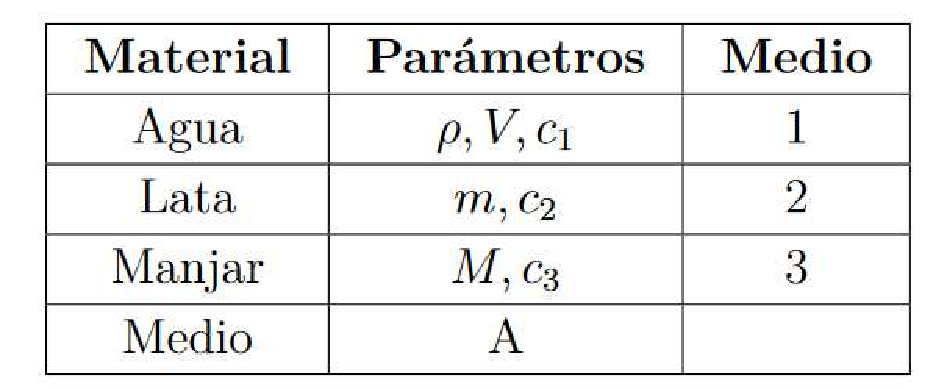
\includegraphics[width=0.3\textwidth]{Auxiliar_1_4}
            \captionof{figure}{Esquema del circuito abierto}
        \end{center}
        \item Por otro lado sea el caso que $R_{2}$ tiende a 0, se tiene que en base al mismo analisis:
        \begin{equation}
            lim_{R_{2} \to 0} (P_{R2}) = \frac{R_{2} \cdot V^{2}}{(R_{1} + R_{2})^{2}} = \frac{0 \cdot V^{2}}{(R_{1})^{2}} = 0
        \end{equation}
        Por otro lado el voltaje se tendra que:
        \begin{equation}
            lim_{R_{2} \to 0} (V_{R2}) = R_{2} \cdot I_{1} = R_{2}\left( \frac{V}{R_{1} + R_{2}} \right) = 0
        \end{equation}
        Por ultimo la corriente se tendra que:
        \begin{equation}
            lim_{R_{2} \to 0} (I_{1}) = \frac{V}{R_{1} + R_{2}} = \frac{V}{R_{1}} = \frac{V}{R_{1}}
        \end{equation}
        Este fenomeno es conocido como un corto circuito, puede entenderse como que la resistencia tiende a 0 y por tanto no permite caida de voltaje y deja pasar toda la corriente, por lo tanto no se disipa potencia.
        \begin{center}
            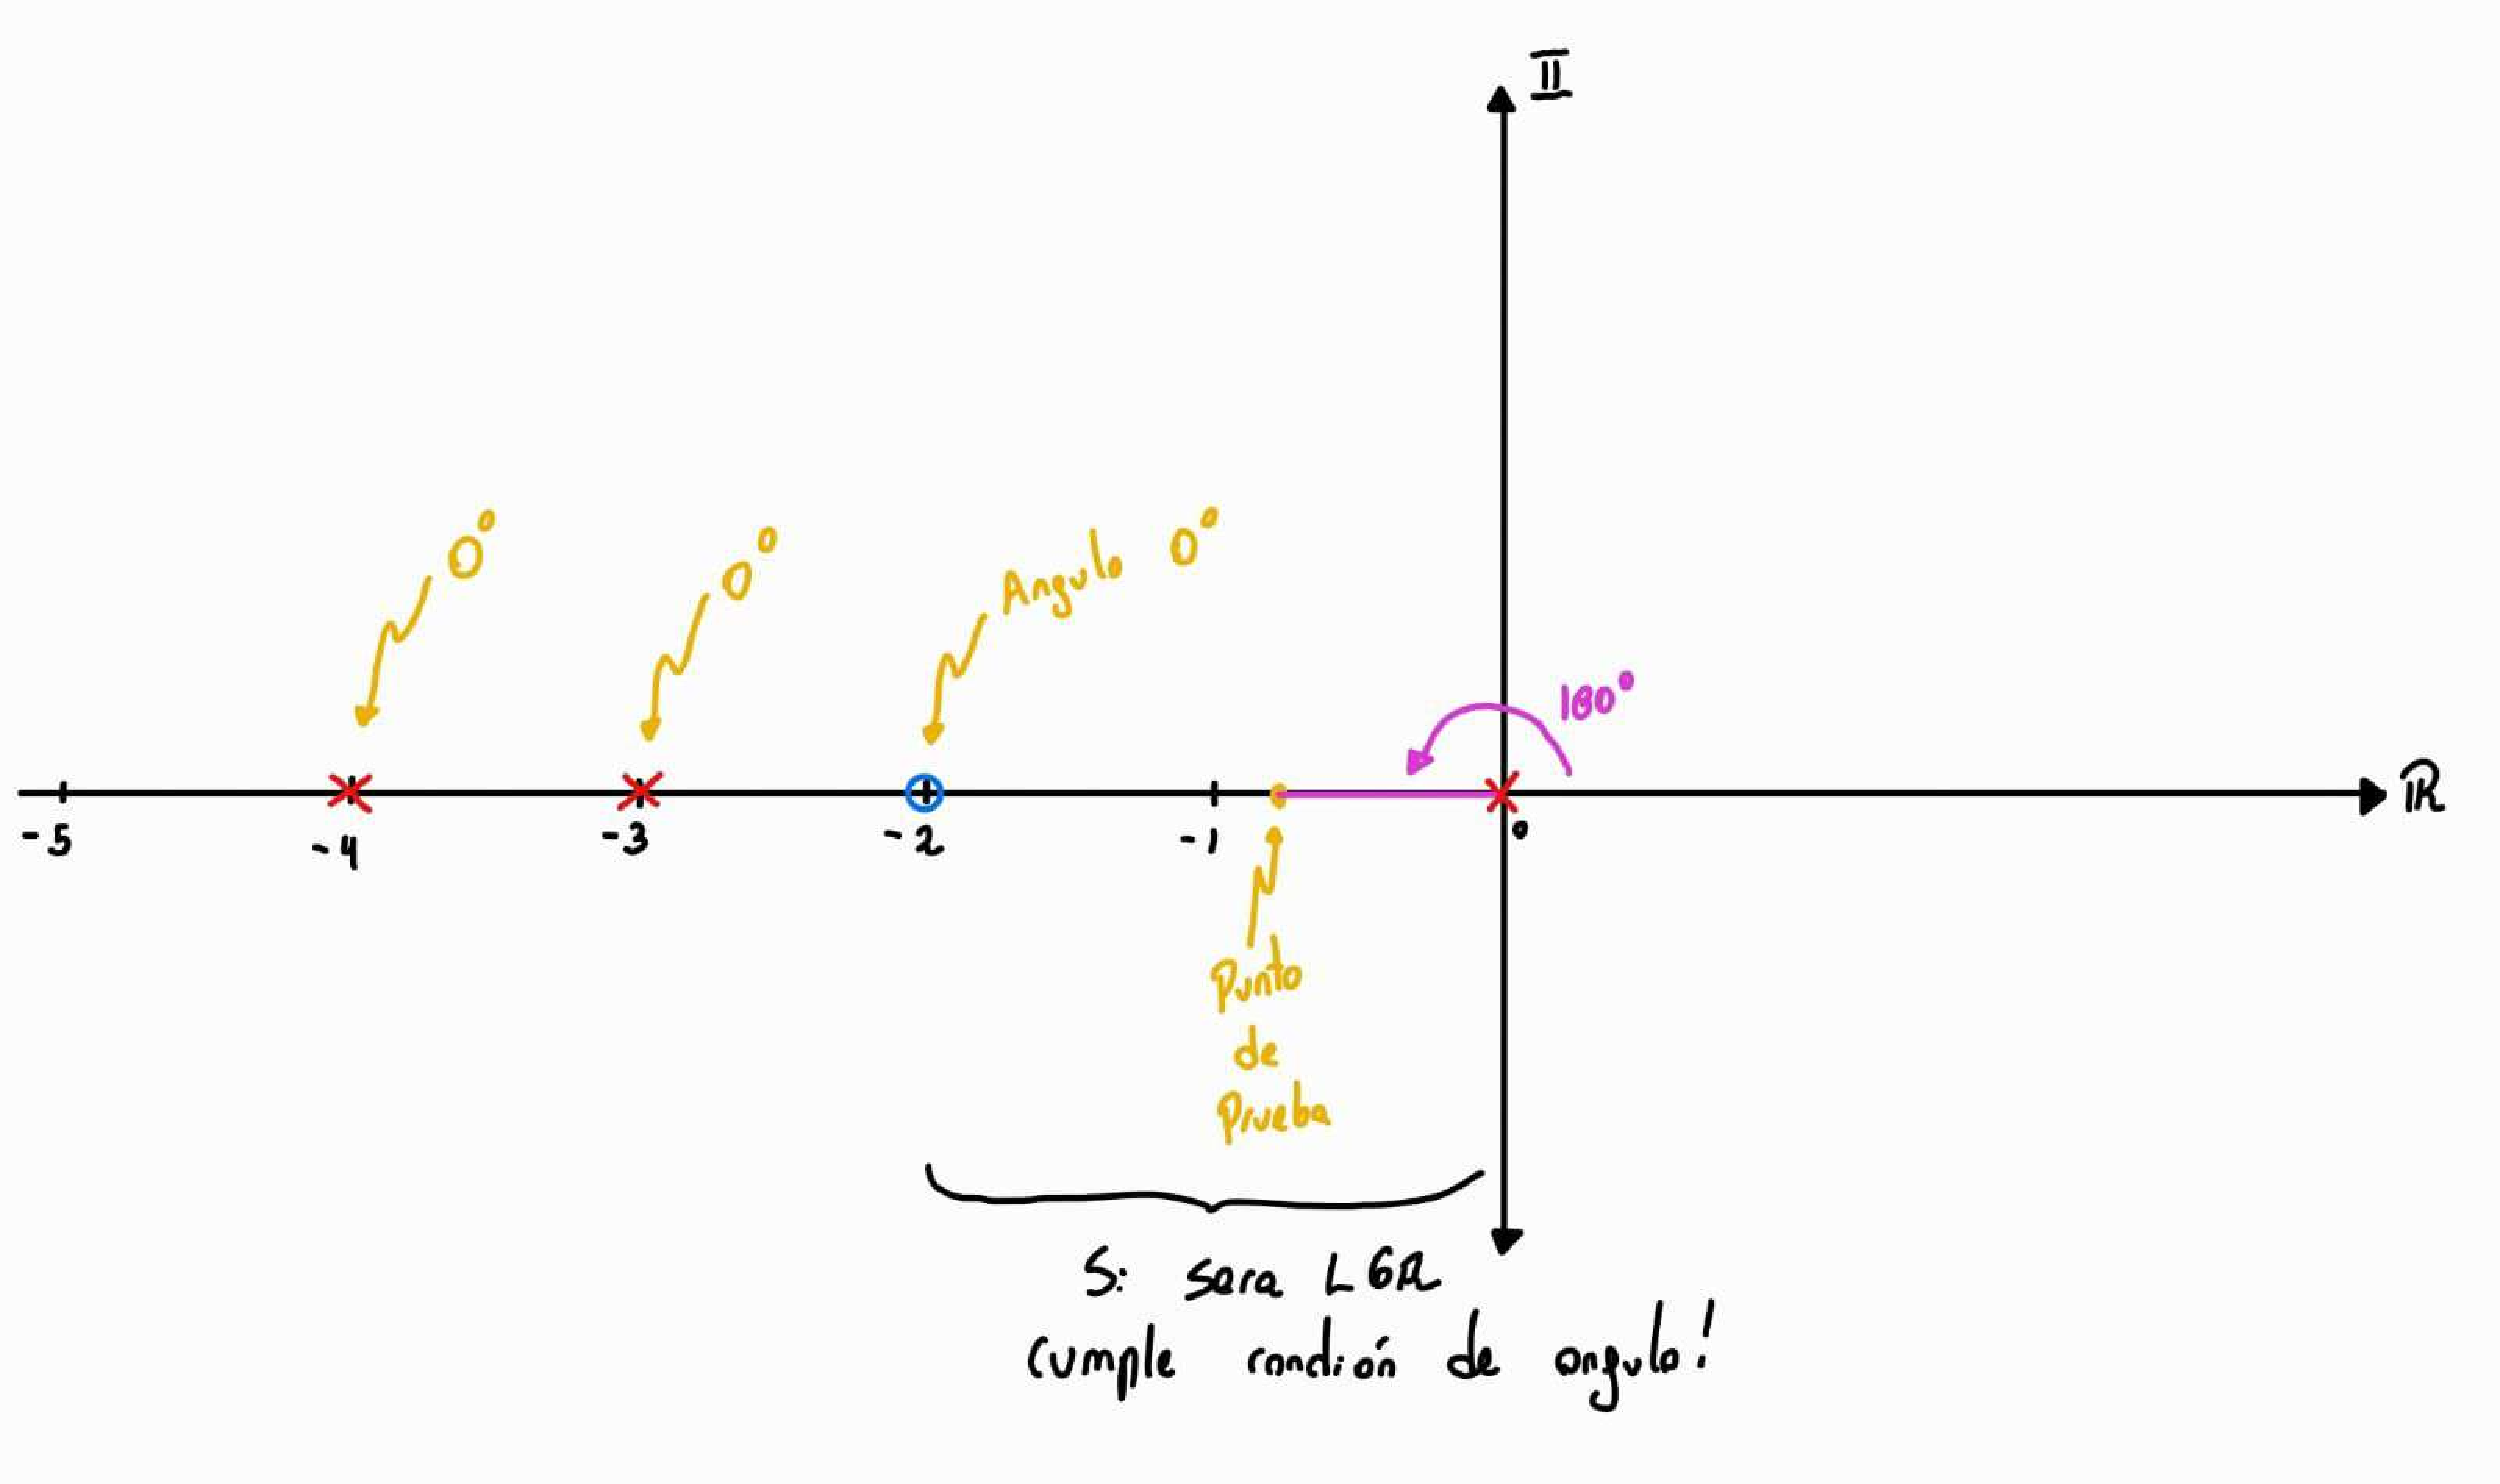
\includegraphics[width=0.4\textwidth]{Auxiliar_1_5}
            \captionof{figure}{Esquema del circuito cerrado para $R_{2}$}
        \end{center}
        Estos dos conceptos es super importante entenderlos y no confundirlos.
    \end{enumerate}
    \end{solution}
%%%%%%%%%%%%%%%%%%%%%%%%%%%
\question  En base a la figura del enunciado:
\begin{enumerate}
    \item Asigne referencias a cada elemento.
    \item Use LVK para encontrar el voltaje en cada resistencia.
    \item Use la ley de Ohm para encontrar la corriente en cada resistencia.
    \item Use LCK para encontrar la corriente que pasa a través de cada fuente de voltaje.
\end{enumerate}
\begin{center}
    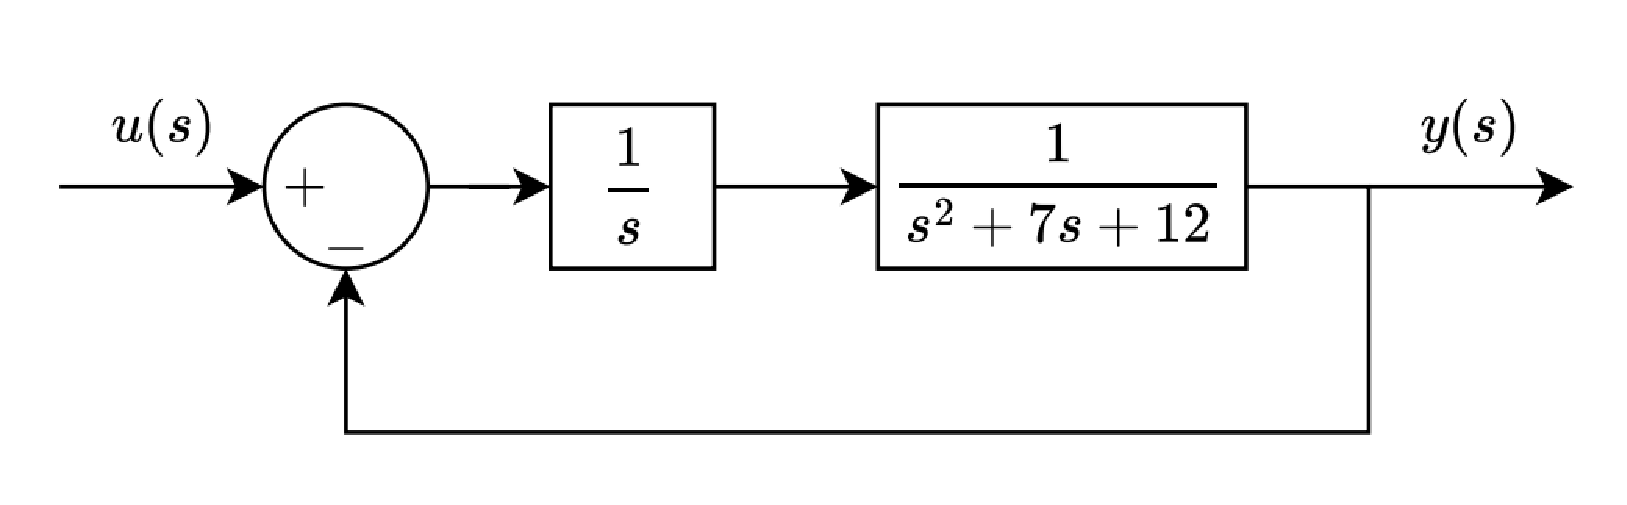
\includegraphics[width=0.5\textwidth]{Auxiliar_1_2}
    \captionof{figure}{Esquema del circuito}
\end{center}
%%%%%%%%%%%%%%%%%%%%%%%%%%%
\begin{solution}
   \begin{enumerate}
    \item Las asignaciones de referencias son arbitrarias y propias de quien las plantee, el unico requerimiento es que se mantenga la consistencia en el analisis, en este caso particular:
    \begin{center}
        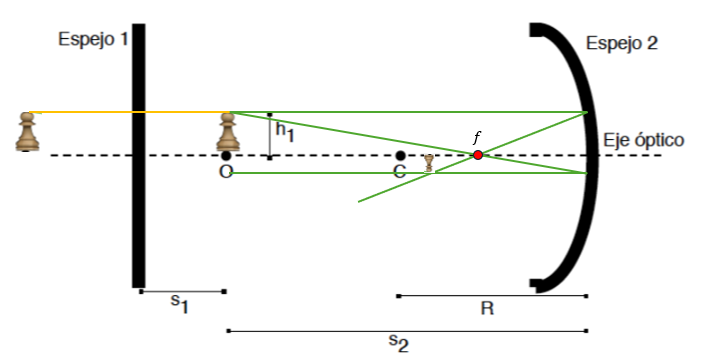
\includegraphics[width=0.5\textwidth]{Auxiliar_1_6}
        \captionof{figure}{Esquema del circuito}
    \end{center}
    \item Se busca obtener el voltaje en cada resistencia, por lo tanto se plantea LVK en cada malla:
    \begin{center}
        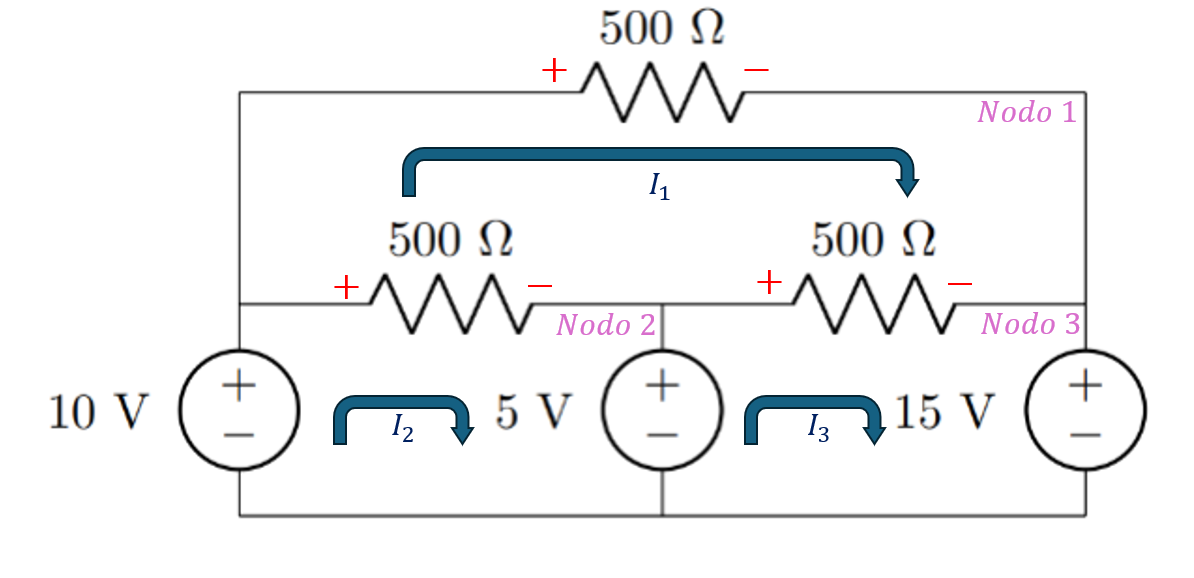
\includegraphics[width=0.6\textwidth]{Auxiliar_1_7}
        \captionof{figure}{Esquema del circuito con todas las referencias}
    \end{center}
    Luego para cada nodo tenemos lo siguiente:
    \begin{align}
        \sum_{\text{Nodo 1}} V_{n} &= V_{1} - V_{2} - V_{3} = 0\\
        V_{1} &= V_{2} + V_{3}
    \end{align}
    \begin{align}
        \sum_{\text{Nodo 2}} V_{n} &= 5[v] - 10[v] + V_{2} = 0\\
        V_{2} &= 5[v]
    \end{align}
    \begin{align}
        \sum_{\text{Nodo 3}} V_{n} &= 15[v] - 5 + V_{3} = 0\\
        V_{3} &= -10[v]
    \end{align}
    Con lo que finalmente se obtiene $V_1 = V_2 + V_3 = -5[v]$
    \item Se busca obtener la corriente en cada resistencia, pero utilizando LCK, para esto tenemos el siguiente esquema:
    \begin{center}
        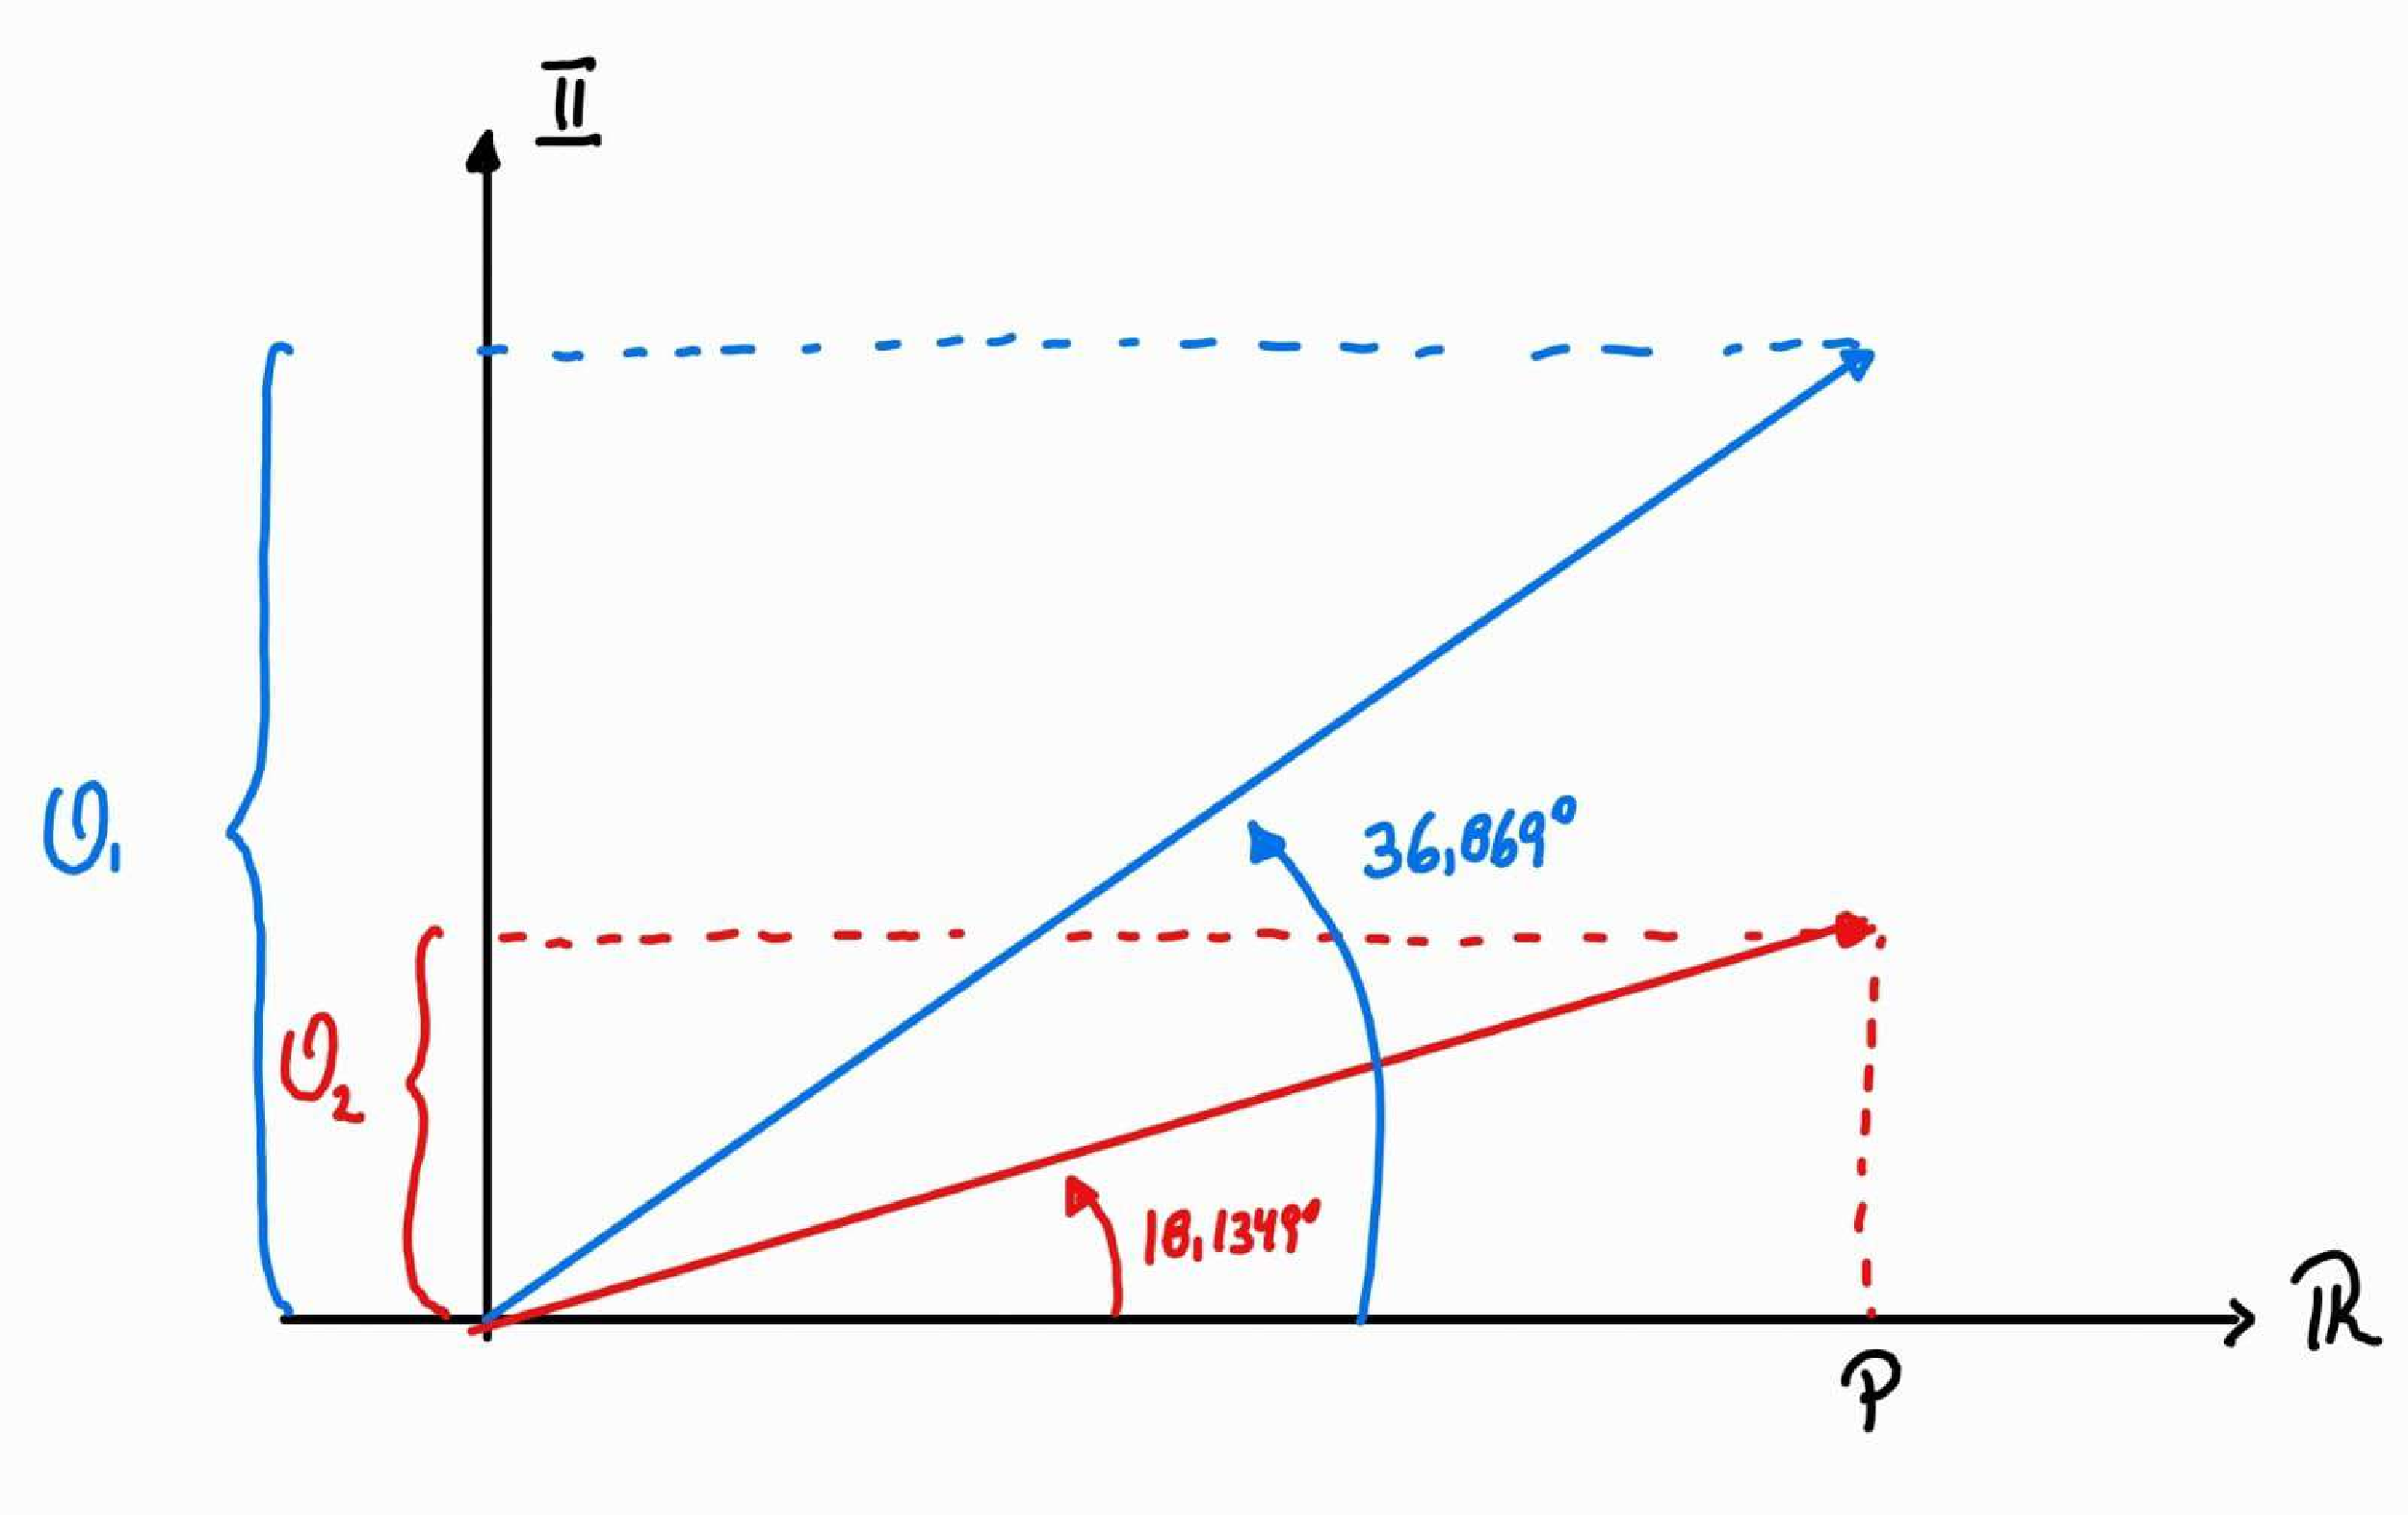
\includegraphics[width=0.5\textwidth]{Auxiliar_1_8}
        \captionof{figure}{Esquema del circuito}
    \end{center}
    Luego se tiene que en cada nodo:
    \begin{align}
    \text{Nodo A:} \quad & i_3 + i_1 = i_2 \\
    \text{Nodo B:} \quad & i_6 + i_2 + i_3 = 0 \\
    \text{Nodo C:} \quad & i_4 = i_3 + i_5
    \end{align}
    Luego se tiene lo siguiente para la diferencia de voltajes:
    \begin{multicols}{2} % Inicia dos columnas

        \begin{align*}
            V_{AB}: V_A - V_B = V_2 &= i_2 R_2 \\
            V_A - V_B &= i_2 R_2 \\
            10[V] - 5[V] &= i_2 R_2 \\
            \frac{5[V]}{500[\Omega]} &= i_2 \\
            i_2 &= 0.01[A]
        \end{align*}
    
        \begin{align*}
            V_{CB} : V_C - V_B &= i_5 R_3 \\
            V_C - V_B &= i_5 R_3 \\
            15[V] - 5[V] &= i_5 R_3 \\
            \frac{10[V]}{500[\Omega]} &= i_5 \\
            i_5 &= 0.02[A]
        \end{align*}
    
        \begin{align*}
            i_6 &= -(i_2 + i_5) \\
            i_6 &= -0.03[A]
        \end{align*}
    
        \columnbreak % Salto a la segunda columna
    
        \begin{align*}
            V_{CA} : V_C - V_A &= i_3 R_1 \\
            15[V] - 10[V] &= i_3 R_1 \\
            i_3 &= \frac{5[V]}{500[\Omega]} \\
            i_3 &= 0.01[A]
        \end{align*}
    
        \begin{align*}
            i_1 &= i_2 - i_3 \\
                &= 0.01[A] - 0.01[A] \\
                &= 0[A]
        \end{align*}
    
        \begin{align*}
            i_5 &= i_4 - i_3 \\
            0.02[A] &= i_4 + 0.01[A] \\
            i_4 &= 0.01[A]
        \end{align*}
    
    \end{multicols}
    


    \end{enumerate}

\end{solution}
%%%%%%%%%%%%%%%%%%%%%%%%%%%
\question En base a la figura del enunciado:
\begin{enumerate}
    \item Identifique todos los nodos.
    \item Simplifique el circuito lo que más pueda y luego asigne referencia de signos.
    \item Plantee todas las ecuaciones de malla del circuito. 
    \item Calcule las corrientes incógnitas del método de mallas considerando que todas las resistencias tienen el mismo valor.
\end{enumerate}
\begin{center}
    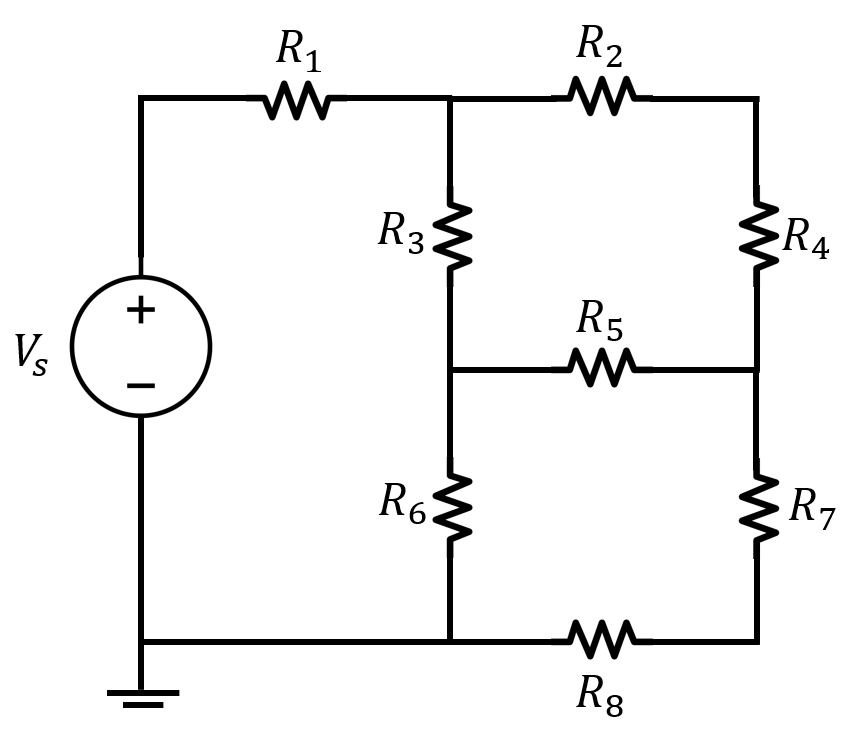
\includegraphics[width=0.5\textwidth]{Auxiliar_1_3}
    \captionof{figure}{Esquema del circuito}
\end{center}
\end{questions}
%%%%%%%%%%%%%%%%%%%%%%%%%%%
\begin{solution}
    \begin{enumerate}
        \item Se busca el identificar todos los nodos del circuito, por lo tanto se tiene lo siguiente:
        \begin{center}
            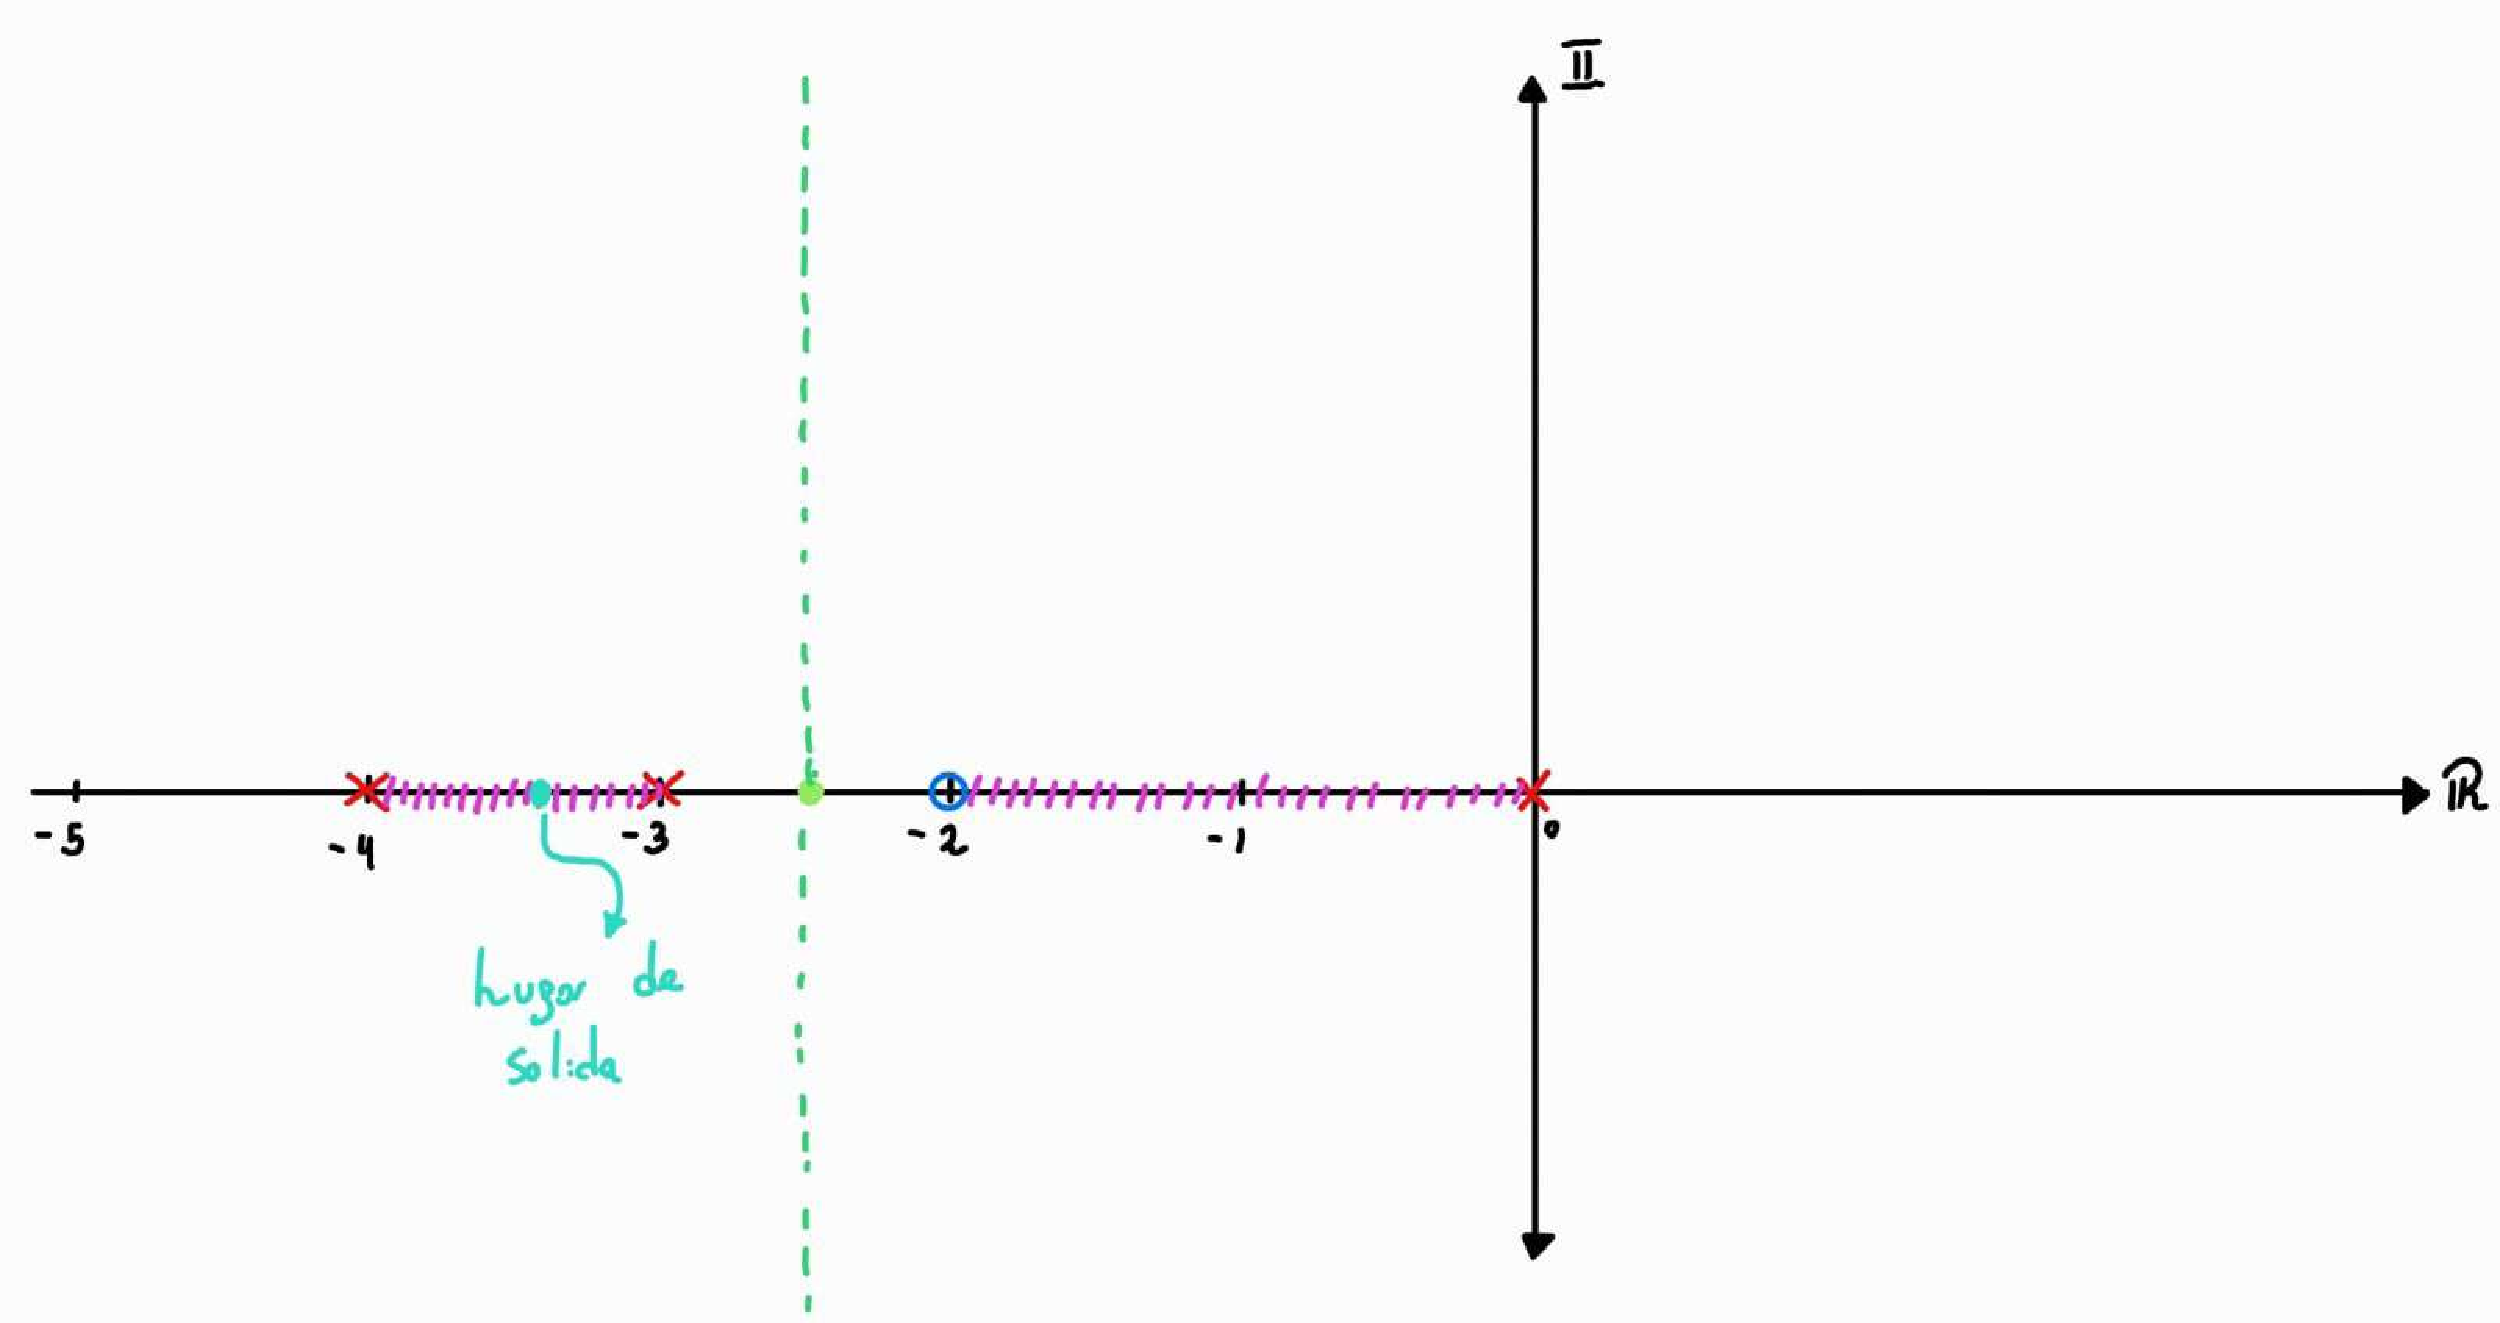
\includegraphics[width=0.4\textwidth]{Auxiliar_1_9}
            \captionof{figure}{Esquema del circuito con los nodos identificados}
        \end{center}
        \item Se busca simplificar el circuito lo mas posible, por lo tanto se identifica lo siguiente:
        \begin{itemize}
            \item Tanto $R_2$ como $R_4$ se encuentran en serie.
            \item Tanto $R_7$ como $R_8$ se encuentran en serie.
        \end{itemize}
        Luego tenemos que el esquema simplificado es el siguiente:
    \begin{center}
        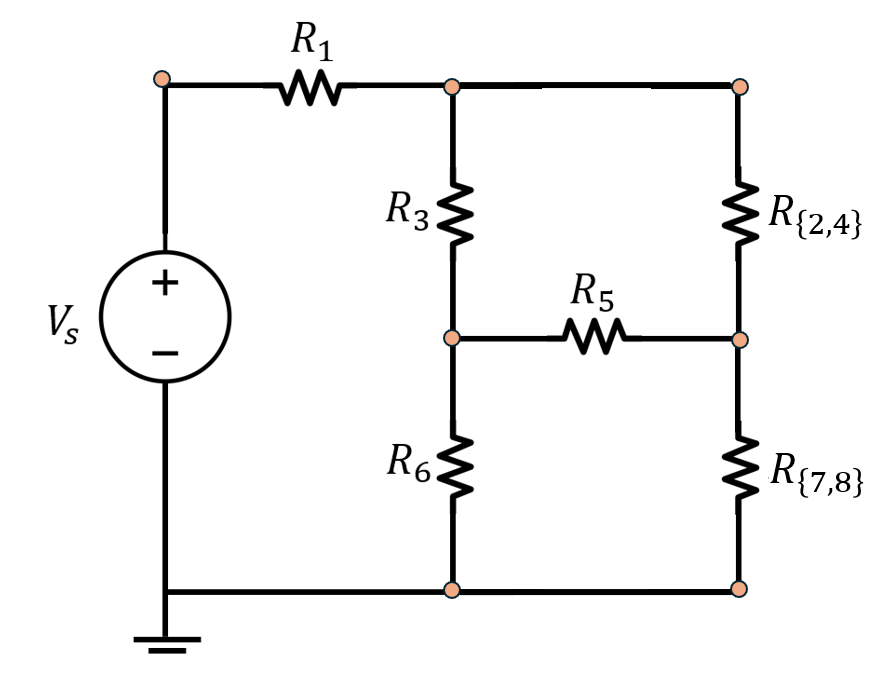
\includegraphics[width=0.4\textwidth]{Auxiliar_1_10}
        \captionof{figure}{Esquema del circuito con los nodos identificados}
    \end{center}
    Luego se asignan las referencias de signos dando como resultado:
    \begin{center}
        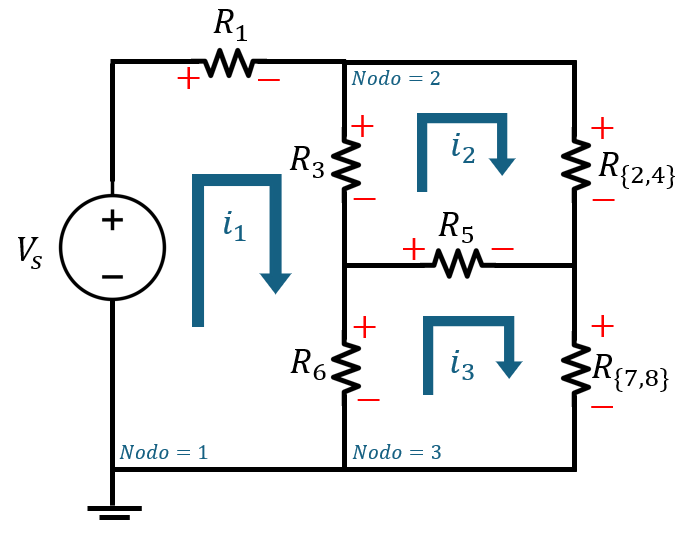
\includegraphics[width=0.4\textwidth]{Auxiliar_1_11}
        \captionof{figure}{Esquema del circuito con los referencias}
    \end{center}
    \item Luego se busca plantear las ecuaciones de malla, por lo tanto se tiene lo siguiente:
    \begin{align}
        \text{Malla 1:} \quad & -V_s + V_1 + V_3 + V_6 = 0 \\
        \text{Malla 2:} \quad & - V_3 + V_{2,4} - V_5 = 0 \\
        \text{Malla 3:} \quad & -V_6 + V_5 - V_{7,8} = 0 
    \end{align}
    Luego reoordenando de manera conveniente tenemos que:
    \begin{align}
        V_s &= V_1 + V_3 + V_6 \\
        0 &= V_3 + V_5 - V_{2,4} \\
        0 &= V_5 + V_{7,8} - V_6 
    \end{align}
    Luego ademas tenemos que:
    \begin{align}
        V_1 &= i_1 R_1 \\
        V_{2,4} &= i_2 R_{2,4}= i_2 (R_2 + R_4) \\
        V_3 &= (i_1 - i_2) R_3 \\
        V_5 &= (i_3 - i_2) R_5 \\
        V_6 &= (i_1 - i_3) R_6 \\
        V_{7,8} &= i_3 R_{7,8} = i_3 (R_7 + R_8)
    \end{align}
    Reemplazando sobre lo anterior tenemos que:
    \begin{align}
        V_s &= V_1 + V_3 + V_6 = i_1 R_1 + (i_1 - i_2) R_3 + (i_1 - i_3) R_6 \\
        0 &= V_3 + V_6 - V_{2,4}= (i_1 - i_2) R_3 + (i_3 - i_2) R_5 - i_2 (R_2 + R_4) \\
        0 &= V_5 + V_{7,8}- V_6 = (i_3 - i_2) R_5 + i_3 (R_7 + R_8) - (i_1 - i_3) R_6 
    \end{align}
    Luego reoordenando se tiene:
    \begin{align}
        V_s &= i_1 (R_1 + R_3 + R_6) + i_2 (-R_3) + i_3 (-R_6) \\
        0 &= i_1 (R_3) + i_2 (-R_5 - R_4 - R_3 - R_2) + i_3 (R_5) \\
        0 &= i_1 (-R_6) + i_2 (-R_5) + i_3 (R_8 + R_7 + R_6 + R_5) 
    \end{align}
    Con lo que expresando en forma matricial tenemos que:
    \begin{equation}
        \begin{bmatrix}
            R_1 + R_3 + R_6 & -R_3 & -R_6 \\
            R_3 & -R_5 - R_4 - R_3 - R_2 & R_5 \\
            -R_6 & -R_5 & R_8 + R_7 + R_6 + R_5
        \end{bmatrix}
        \begin{bmatrix}
            i_1 \\
            i_2 \\
            i_3
        \end{bmatrix}
        =
        \begin{bmatrix}
            V_s \\
            0 \\
            0
        \end{bmatrix}
    \end{equation}
    Luego multiplicando por (-1) la segunda fila se obtiene:
    \begin{equation}
        \begin{bmatrix}
            R_1 + R_3 + R_6 & -R_3 & -R_6 \\
            -R_3 & R_5 + R_4 + R_3 + R_2 & -R_5 \\
            -R_6 & -R_5 & R_8 + R_7 + R_6 + R_5
        \end{bmatrix}
        \begin{bmatrix}
            i_1 \\
            i_2 \\
            i_3
        \end{bmatrix}
        =
        \begin{bmatrix}
            V_s \\
            0 \\
            0
        \end{bmatrix}
    \end{equation}
    En base al enunciado, se consideran todas las resistencias iguales por tanto:
    \begin{equation}
        \begin{bmatrix}
            3R & -R & -R \\
            -R & 4R & -R \\
            -R & -R & 4R
        \end{bmatrix}
        \begin{bmatrix}
            i_1 \\
            i_2 \\
            i_3
        \end{bmatrix}
        =
        \begin{bmatrix}
            V_s \\
            0 \\
            0
        \end{bmatrix}
    \end{equation}
    Por lo que se necesita obtener la inversa de la matriz de coeficientes (\textbf{Propuesta para el lector}), por tanto se tiene:
    \begin{equation}
        \begin{bmatrix}
            3R & -R & -R \\
            -R & 4R & -R \\
            -R & -R & 4R
        \end{bmatrix}^{-1}
        =
        \begin{bmatrix}
            3/7R & 1/7R & 1/7R \\
            1/7R & 11/35R & 4/35R \\
            1/7R & 4/35R & 11/35R
        \end{bmatrix}
    \end{equation}
    De esta manera tenemos que las corrientes vendran dadas por:
    \begin{equation}
        \begin{bmatrix}
            i_1 \\
            i_2 \\
            i_3
        \end{bmatrix}
        =
        \begin{bmatrix}
            3/7R & 1/7R & 1/7R \\
            1/7R & 11/35R & 4/35R \\
            1/7R & 4/35R & 11/35R
        \end{bmatrix}
        \begin{bmatrix}
            V_s \\
            0 \\
            0
        \end{bmatrix}
    \end{equation}
    De esta manera se tiene que las corrientes seran:
    \begin{align}
        i_1 &= \frac{3}{7R} \cdot V_s \\
        i_2 &= \frac{1}{7R} \cdot V_s \\
        i_3 &= \frac{1}{7R} \cdot V_s
    \end{align}
    Con lo que se obtienen las corrientes incognitas del circuito.
    \end{enumerate}
\end{solution}
\end{document}